\documentclass[no-math]{ctexrep}
\usepackage[hmargin=1.25in,vmargin=1in]{geometry}
\usepackage{multirow}
\usepackage{graphicx}
\usepackage{fontspec}
\usepackage{xcolor}
\usepackage{subfig}
\usepackage[chapter]{minted}
\usepackage[colorlinks=true,bookmarks=true,bookmarksnumbered=true]{hyperref}

\definecolor{mintbg}{rgb}{0.95,0.95,0.95}
\renewcommand{\listingscaption}{源代码}

\setmonofont{WenQuanYi Micro Hei Mono}

\author{71120226 陈宇轩}
\title{数据结构实验五:树\ 实验报告}

\begin{document}
    \maketitle

    \tableofcontents

    \chapter{题目一}

    \section{题目描述}

    给定一棵结点数为 $n$ 的二叉树,求该树的深度。树的深度定义为其所有结点深度的最大值。

    \subsection{输入输出格式}

    \subsubsection{输入格式}

    输入共包含 $n + 1$ 行:

    \begin{itemize}
        \item 第一行包含两个正整数 $n, rt$,依次代表给定树的结点数量,树的根;
        \item 接下来第 $2$ 至第 $n + 1$ 行,第 $i$ 行有 2 个非负整数,依次代表结点 $i - 1$ 的左右子结点编号;
        \begin{itemize}
            \item 特别地,0 表示该子结点为空(不存在)。
        \end{itemize}
    \end{itemize}

    输入保证所有结点恰好构成一棵二叉树。

    \subsubsection{输出格式}

    输出仅包含一行,包含一个整数,代表给定树的深度。

    \subsubsection{输入输出样例}

    \begin{tabular}{|c|l|l|}
        \hline
        样例编号 & 样例输入 & 样例输出 \\ \hline
        \multirow{2}{*}{1} & \mintinline{text}{1 1} & \mintinline{text}{1} \\
         & \mintinline{text}{0 0} & \\ \hline
        \multirow{6}{*}{2} & \mintinline{text}{5 1} & \mintinline{text}{3} \\
         & \mintinline{text}{2 3} & \\
         & \mintinline{text}{4 5} & \\
         & \mintinline{text}{0 0} & \\
         & \mintinline{text}{0 0} & \\
         & \mintinline{text}{0 0} & \\ \hline
    \end{tabular}

    \subsection{数据范围}

    $1 \le n \le 10,\!000$

    \section{思路分析}

    输入输出略。

    考虑直接使用 DFS 来完成任务。DFS 的每一层调用栈对应原树的一个结点,则每当访问当前结点的子结点时,深度 +1。由于实现中结点并不保存自身的深度,在函数调用中我们必须额外传递一个参数来记录当前结点的深度。最后直接返回两个子结点的最大深度(如果当前为叶子结点,则直接返回自身深度)即可。

    \section{源码}

    见 \mintinline{text}{p1.cpp}。

    \section{运行截图}

    见图 \ref{figure:p1}。

    \begin{figure}[hp]
        \centering
        \caption{实验一 运行截图}
        \label{figure:p1}
        \subfloat[样例一]{
            \centering
            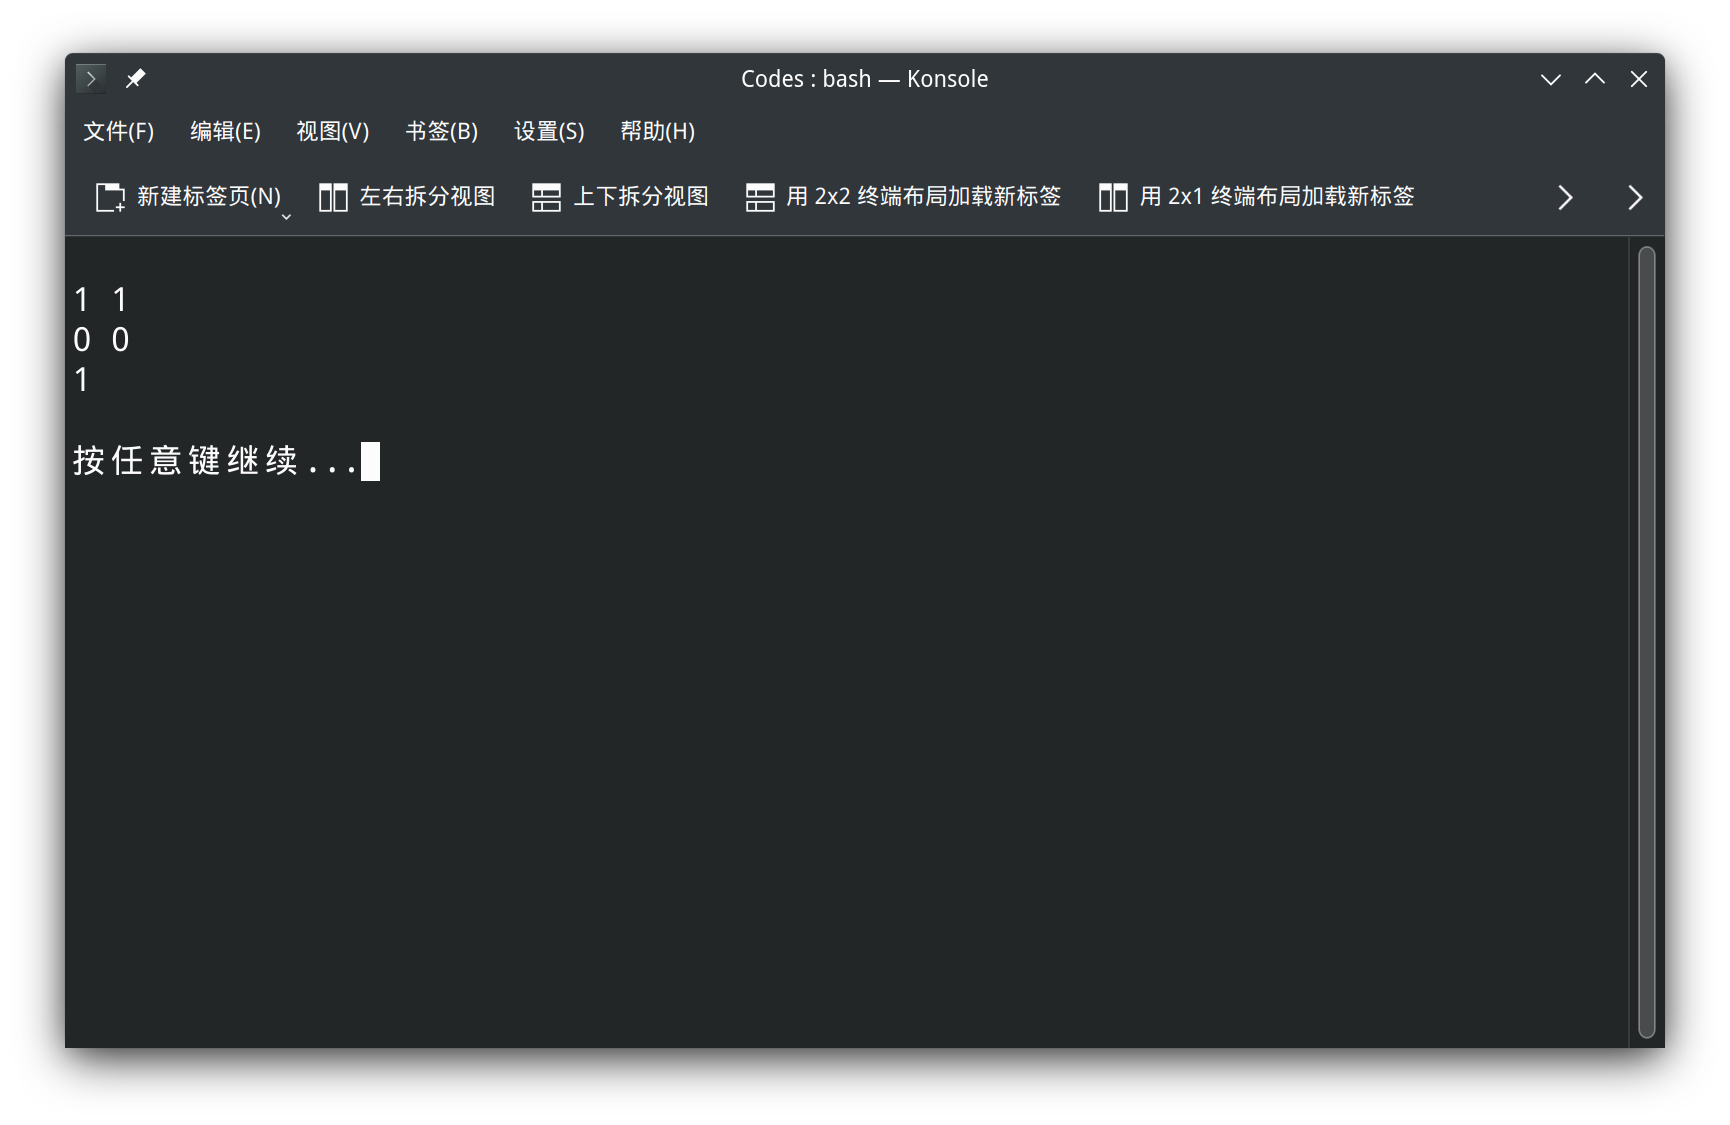
\includegraphics[scale=0.3]{pics/p1-1.png}
        }
        \newline
        \subfloat[样例二]{
            \centering
            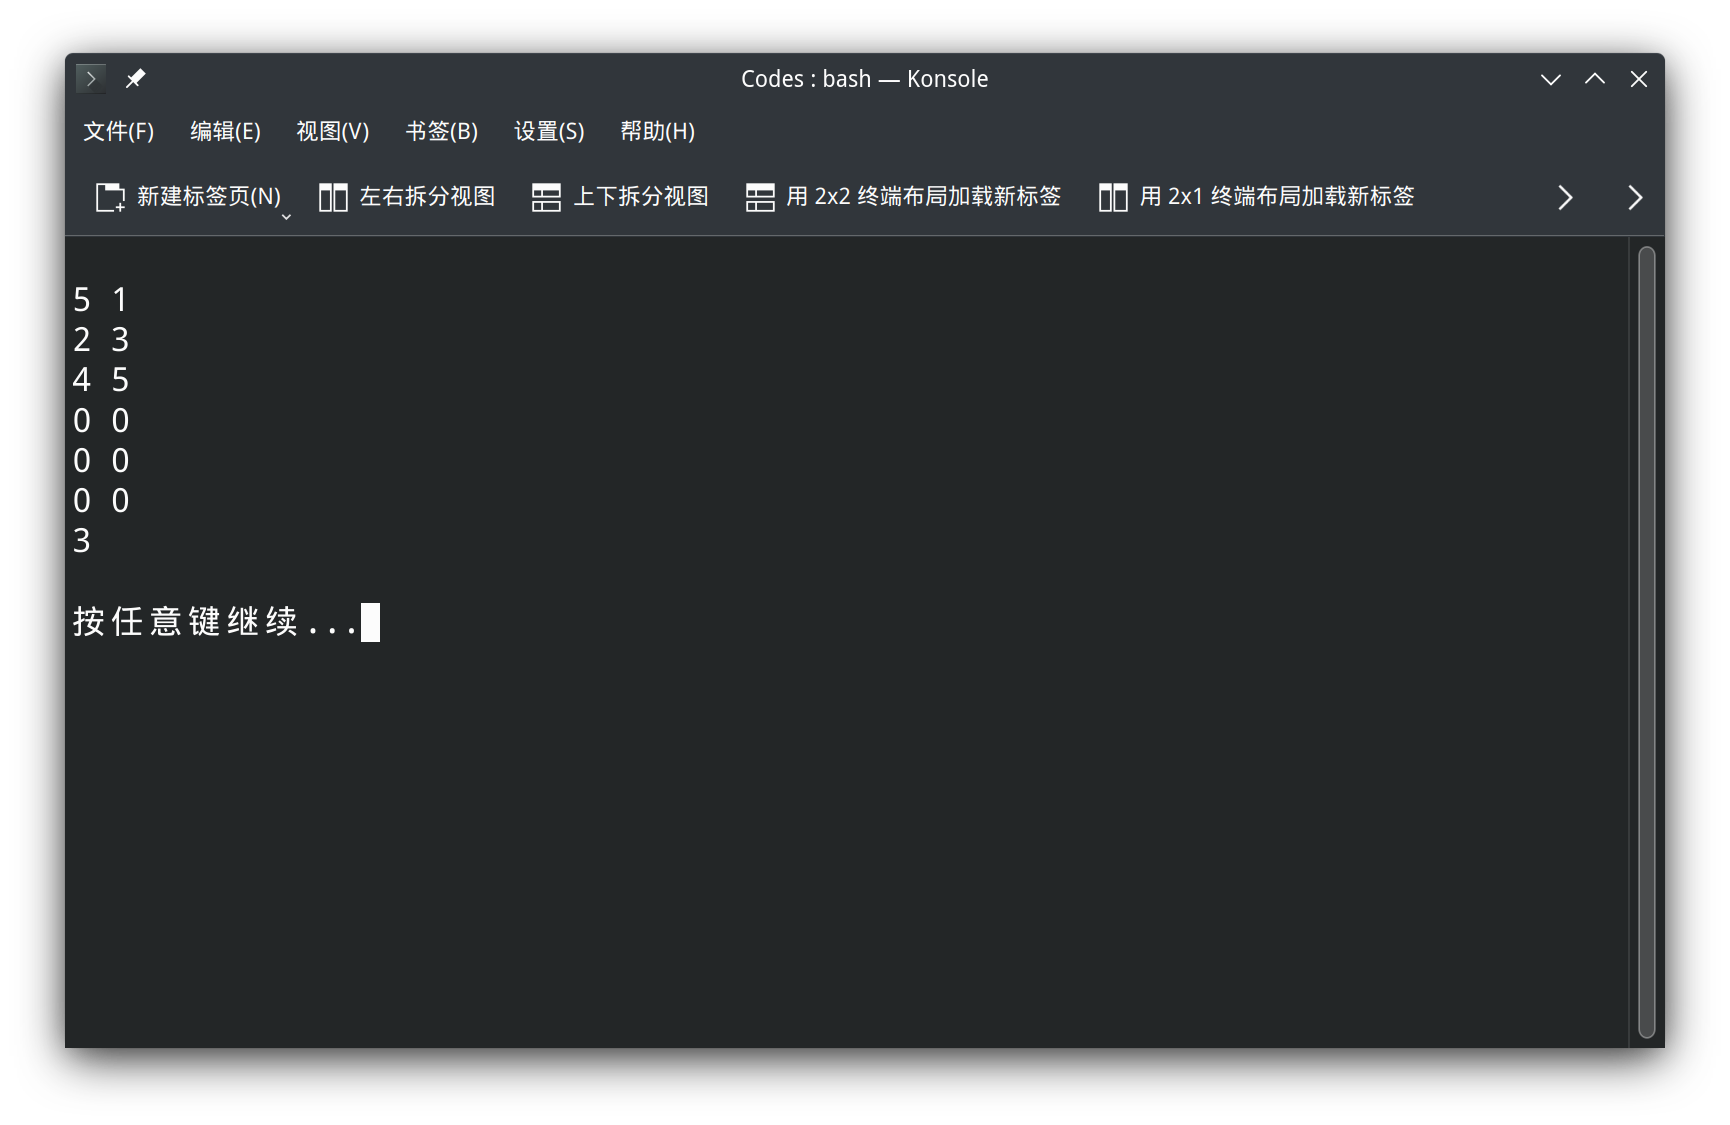
\includegraphics[scale=0.3]{pics/p1-2.png}
        }
    \end{figure}

\end{document}